\documentclass[12pt, twoside]{article}
\input{../preamble}

\fancyhead[LO]{La Scuola d'Italia / Dr.\ Huson / IB Math: Probability \\* 13 March 2026}
\fancyhead[RO]{\fbox{\begin{minipage}{6cm}\footnotesize First \& Last name:\\[0.5cm]\end{minipage}}}
\fancyfoot[C]{\thepage}

\begin{document}
\subsubsection*{4.19 Quiz: Probability Review}

\begin{enumerate}[itemsep=0.1cm]

%--- Problem 1: Venn diagram reading ---
\item In a class of 32 students, some do Music ($M$) and some do Drama ($D$).

\begin{center}
\vspace{-0.3cm}
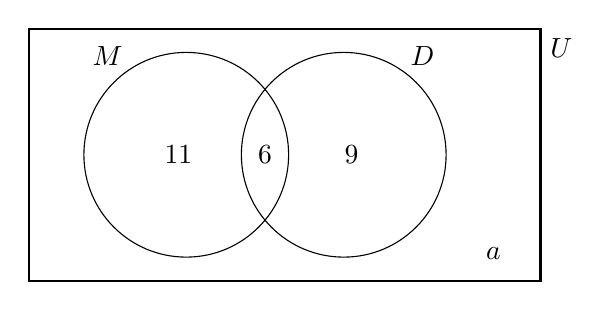
\begin{tikzpicture}
  \draw[thick] (0,0) rectangle (6.5,3.2);
  \node[anchor=north west] at (6.5,3.2) {$U$};
  \draw (2.0,1.6) circle (1.3cm);
  \node at (1.0,2.85) {$M$};
  \draw (4.0,1.6) circle (1.3cm);
  \node at (5.0,2.85) {$D$};
  \node at (1.9,1.6) {$11$};
  \node at (3.0,1.6) {$6$};
  \node at (4.1,1.6) {$9$};
  \node at (5.9,0.35) {$a$};
\end{tikzpicture}
\vspace{-0.3cm}
\end{center}

\begin{enumerate}[itemsep=0.1cm]
  \item Write down the number of students who do Music. \hfill [1]
  \item Find the number of students who do neither Music nor Drama, $a$. \hfill [1]
  \item One student is chosen at random. Find the probability that
  \begin{enumerate}[label=(\roman*), itemsep=0.1cm]
    \item the student does not do Music; \hfill [1]
    \item the student does Music or Drama, but not both. \hfill [2]
  \end{enumerate}
  \item Given that a student does Drama, find the probability that they also do Music. \hfill [2]
\end{enumerate}

\begin{tikzpicture}
  \draw (-0.6,0) rectangle (11,12);
  \foreach \y in {1,2,3,4,5,6,7,8,9,10,11} \draw[dotted] (0,\y)--(10.5,\y);
\end{tikzpicture}

\newpage

%--- Problem 2: Two-way table + independence ---
\item The following table shows whether 16 students are in the IB math program
and whether they have a TI nSpire calculator.

\renewcommand{\arraystretch}{1.4}
\begin{center}
\begin{tabular}{|r|c|c|c|}
    \hline
    & nSpire & No nSpire & Total \\
    \hline
    IB        & 8  & 2  & 10 \\
    \hline
    Non-IB    & 1  & 5  & 6 \\
    \hline
    Total     & 9  & 7  & 16 \\
    \hline
\end{tabular}
\end{center}

\begin{enumerate}[itemsep=0.0cm]
  \item Find the probability that a randomly chosen student is in IB
        and has a nSpire. \hfill [1]
  \item Find $\mathrm{P}(\text{nSpire} \mid \text{non-IB})$. \hfill [2]
  \item Determine whether ``is in IB'' and ``has a nSpire'' are
        independent events.
        Show your working and justify your answer. \hfill [3]
\end{enumerate}

\begin{tikzpicture}
  \draw (-0.6,0) rectangle (11,11);
  \foreach \y in {1,2,3,4,5,6,7,8,9,10,11} \draw[dotted] (0,\y)--(10.5,\y);
\end{tikzpicture}

\newpage
%--- Problem 3: Tree diagram ---
\item At a school, 60\% of students take the bus and 40\% walk.
Of those who take the bus, 10\% arrive late.
Of those who walk, 5\% arrive late.

\begin{enumerate}[itemsep=0.2cm]
  \item Complete the tree diagram below, showing all probabilities. \hfill [2]
    \vspace{1cm}
  \begin{flushleft}
  \vspace{-0.2cm}
  \begin{tikzpicture}[xscale=1, yscale=1]
    % Main branches
    \draw (0,0) -- (3.5, 1.8);
    \draw (0,0) -- (3.5,-1.8);
    % Bus branches
    \draw (3.5, 1.8) -- (7.0, 2.8);
    \draw (3.5, 1.8) -- (7.0, 1.1);
    % Walk branches
    \draw (3.5,-1.8) -- (7.0,-1.1);
    \draw (3.5,-1.8) -- (7.0,-2.8);
    % First-level labels
    \node[above] at (1.75, 0.9) {$0.6$};
    \node[below] at (1.75,-1.9) {\rule{1cm}{0.4pt}};
    \node[above left] at (3.5, 1.8) {\small Bus};
    \node[below left] at (3.7,-2) {\small Walk};
    % Second-level labels
    \node[above] at (5.25, 2.3) {$0.10$};
    \node[below] at (5.25, 0.7) {\rule{1cm}{0.4pt}};
    \node[above] at (5.25,-1.5) {\rule{1cm}{0.4pt}};
    \node[below] at (5.25,-3.0) {\rule{1cm}{0.4pt}};
    % Outcome labels
    \node[anchor=west] at (7.15, 2.8) {Late};
    \node[anchor=west] at (7.15, 1.1) {On time};
    \node[anchor=west] at (7.15,-1.1) {Late};
    \node[anchor=west] at (7.15,-2.8) {On time};
    % Compound probability blanks
    \node[anchor=west] at (9.5, 2.8) {$=$ \rule{1.5cm}{0.4pt}};
    \node[anchor=west] at (9.5, 1.1) {$=$ \rule{1.5cm}{0.4pt}};
    \node[anchor=west] at (9.5,-1.1) {$=$ \rule{1.5cm}{0.4pt}};
    \node[anchor=west] at (9.5,-2.8) {$=$ \rule{1.5cm}{0.4pt}};
  \end{tikzpicture}
  \vspace{-0.2cm}
  \end{flushleft}

  \item Find the probability that a randomly chosen student walks and
        arrives late. \hfill [1]
  \item Find the probability that a randomly chosen student arrives late. \hfill [2]
  \item Given that a student arrives late, find the probability that they walk. \hfill [2]
\end{enumerate}

\begin{tikzpicture}
  \draw (-0.6,0) rectangle (11,10);
  \foreach \y in {1,2,3,4,5,6,7,8,9,10} \draw[dotted] (0,\y)--(10.5,\y);
\end{tikzpicture}

\newpage
%--- Problem 4: Without replacement ---
\item A bag contains 4 black marbles and 6 white marbles. Two marbles are
drawn at random, one after the other, without replacement.

\begin{enumerate}[itemsep=0.1cm]
  \item Find the probability that both marbles are black. \hfill [2]
  \item Find the probability that both marbles are the same colour. \hfill [3]
  \item Find the probability that both marbles are black given that
        at least one marble is black. \hfill [3]
\end{enumerate}

\begin{tikzpicture}
  \draw (-0.6,0) rectangle (11,12);
  \foreach \y in {1,2,3,4,5,6,7,8,9,10,11} \draw[dotted] (0,\y)--(10.5,\y);
\end{tikzpicture}

\end{enumerate}
\end{document}

Solutions
  Problem 1 — Venn diagram reading:
  - (a) n(M) = 11 + 6 = 17
  - (b) a = 32 - 11 - 6 - 9 = 6
  - (c)(i) P(not Music) = (9 + 6)/32 = 15/32
  - (c)(ii) P(Music or Drama, not both) = (11 + 9)/32 = 20/32 = 5/8
  - (d) P(M | D) = 6/15 = 2/5

  Problem 2 — Two-way table + independence:
  - (a) P(IB ∩ nSpire) = 8/16 = 1/2
  - (b) P(nSpire | non-IB) = 1/6
  - (c) P(IB) × P(nSpire) = 10/16 × 9/16 = 90/256 = 0.3516
        P(IB ∩ nSpire) = 8/16 = 0.5
        0.3516 ≠ 0.5 → not independent

  Problem 3 — Tree diagram:
  - (a) Walk = 0.4; Bus on time = 0.90; Walk late = 0.05; Walk on time = 0.95
        Compound: 0.6×0.10 = 0.06; 0.6×0.90 = 0.54; 0.4×0.05 = 0.02; 0.4×0.95 = 0.38
  - (b) P(walk and late) = 0.4 × 0.05 = 0.02
  - (c) P(late) = 0.06 + 0.02 = 0.08
  - (d) P(walk | late) = 0.02/0.08 = 0.25

  Problem 4 — Without replacement (4 black, 6 white):
  - (a) P(both black) = 4/10 × 3/9 = 12/90 = 2/15
  - (b) P(same colour) = P(BB) + P(WW) = 2/15 + (6/10 × 5/9) = 2/15 + 30/90 = 2/15 + 1/3 = 7/15
  - (c) P(at least one black) = 1 - P(WW) = 1 - 1/3 = 2/3
        P(BB | at least one black) = (2/15)/(2/3) = 1/5
